\documentclass[12pt,a4paper,fontset=fandol]{ctexart}

% === 页面设置 ===
\usepackage[top=2.5cm, bottom=2.5cm, left=2.5cm, right=2.5cm]{geometry}
\usepackage{amsmath,amssymb,amsthm}
\usepackage{tikz}
\usetikzlibrary{automata,positioning,arrows,shapes}
\usepackage[edges]{forest}
\usepackage{graphicx}
\usepackage{enumitem}
\usepackage{booktabs}
\usepackage{multirow}
\usepackage{array}
\usepackage{hyperref}
\usepackage{fancyhdr}

\setlength{\headheight}{14.5pt}
\pagestyle{fancy}
\fancyhf{}
\fancyhead[L]{2023年《编译原理》B卷 解答}
\fancyhead[R]{中山大学 计算机学院}
\fancyfoot[C]{\thepage}

\setlength{\parskip}{0.3em}
\setlength{\parindent}{0pt}

\title{\bfseries 2022学年第2学期《编译原理》(B卷) 参考答案与解析}
\author{}
\date{}

\begin{document}

\maketitle
\thispagestyle{fancy}

% ============================================================
% 第一部分：参考答案（简答版）
% ============================================================
\part*{第一部分：参考答案}

\section*{一、判断题（共10小题，每小题1分，共10分）}

\begin{enumerate}[label=\arabic*.]
    \item \textbf{×（错误）。} DFA虽然不允许$\varepsilon$变迁，但只要初始状态同时也是接受状态，即可识别空串$\varepsilon$。识别$\varepsilon$不需要$\varepsilon$变迁。
    \item \textbf{$\checkmark$ （正确）。} 通过子集构造法（Subset Construction），任意NFA都可构造一个等价的DFA。
    \item \textbf{×（错误）。} 文法$A \to Ba \mid a,\; B \to A$存在间接左递归：$A \Rightarrow Ba \Rightarrow Aa$。
    \item \textbf{×（错误）。} 分析树的叶节点可能为$\varepsilon$（空串），$\varepsilon$不是终结符。当文法含$\varepsilon$-产生式时叶节点可为$\varepsilon$。
    \item \textbf{$\checkmark$ （正确）。} LL(0)意味着不向前看任何符号，每个非终结符至多只有一个候选产生式，因此最多产生一个句子。
    \item \textbf{×（错误）。} LALR(1)合并同心项集可能产生新的归约--归约冲突，但\textbf{不会}产生新的移进--归约冲突。
    \item \textbf{×（错误）。} L-属性定义也可在自底向上的LR分析中实现，可通过扩充分析栈来支持。
    \item \textbf{$\checkmark$ （正确）。} 回填（Backpatching）正是用于解决一遍扫描时跳转目标尚未确定的问题。
    \item \textbf{×（错误）。} 全局优化指在一个过程\textbf{内部}跨基本块的优化；跨多个子程序的优化称为过程间优化（Inter-procedural Optimization）。
    \item \textbf{×（错误）。} 指令选择、指令调度、寄存器分配属于\textbf{目标代码生成}阶段，而非中间代码优化阶段。
\end{enumerate}

\section*{二、填空题（共7小题10个空，每空1分，共10分）}

\begin{enumerate}[label=\arabic*.]
    \item \textbf{上下文有关文法 / 1型文法（Type 1, CSG）}
    \item \textbf{$\varepsilon$,\; a,\; aa,\; aac,\; aacB}（含句柄非全长前缀或句柄正在形成的前缀均可）
    \item 第一空：\textbf{$\text{FIRST}(\alpha) \cap \text{FIRST}(\beta) = \varnothing$}；第二空：\textbf{$\text{FIRST}(\beta) \cap \text{FOLLOW}(A) = \varnothing$}
    \item 第一空：\textbf{$n+1$}（$n$个终结符 + \$）；第二空：\textbf{$m$}（$m$个非终结符，不含$S'$）
    \item 第一空：\textbf{$B$为真时控制流转向的代码标号（即$S_1$第一条指令的标号）}；第二空：\textbf{$S$执行完毕后下一条指令的标号}
    \item \textbf{引用计数法（Reference Counting）}
    \item \textbf{6}（LD 读内存 2 + ADD 含内存操作数 2 + ST 写内存 2）
\end{enumerate}

\section*{三、简答题（简要答案）}

\subsection*{第1题}
有二义性。句子 \texttt{id - id - id} 可构造两棵不同的分析树：(id $-$ id) $-$ id 与 id $-$ (id $-$ id)。

\subsection*{第2题}
\textbf{2.1} $T.\textit{type}$为综合属性；$L.\textit{type}$为继承属性。

\textbf{2.2} 带注释分析树（略，见详细解答）。

\subsection*{第3题}
基本块划分：
\begin{itemize}
    \item $B_1 = \{1, 2\}$（入口-出口型）
    \item $B_2 = \{3, 4\}$（条件跳转）
    \item $B_3 = \{5, 6, 7\}$（无条件跳转）
    \item $B_4 = \{8, 9\}$（程序终止）
\end{itemize}
流图：$B_1 \to B_2,\; B_2 \to B_4,\; B_2 \to B_3,\; B_3 \to B_2$。

\subsection*{第4题}
利用DAG消除公共子表达式和死代码后的优化结果：
\begin{verbatim}
    S3 := X - Y
    S4 := X + Y
    A  := 4 * S4
    B  := S3 * S4
\end{verbatim}

\section*{四、应用题（简要答案）}

\subsection*{第1题}
\textbf{1.1} $\; b^*(ab^*ab^*ab^*)^*b^* \;$ 或 $\; (b^*ab^*ab^*a)^*b^*$

\textbf{1.2} DFA含3个状态：$q_0$（初始且接受），$q_1$，$q_2$。转换：$q_0\xrightarrow{a}q_1,\; q_0\xrightarrow{b}q_0;\; q_1\xrightarrow{a}q_2,\; q_1\xrightarrow{b}q_1;\; q_2\xrightarrow{a}q_0,\; q_2\xrightarrow{b}q_2$。

\subsection*{第2题}
\textbf{2.2} G1含左递归$A \to Ab$，不适合自顶向下分析。
G2：$S \to ABa,\; A \to bA \mid \varepsilon,\; B \to dB \mid c$。

\textbf{2.3} FIRST/FOLLOW见详细解答。

\textbf{2.4} G2为LL(1)文法。

\subsection*{第3题}
\textbf{3.1} G3：(0)$S'\to S$, (1)$S\to E+T$, (2)$E\to (E)$, (3)$E\to a$, (4)$T\to b$。

\textbf{3.5} LR(0)存在移进--归约冲突；SLR(1)可解决（因$\text{FOLLOW}(T)=\{\$\}$，与移进符号不相交）。

\textbf{3.6} LR(1)为每个项目附加前瞻符，比SLR(1)的FOLLOW集更精确。


\newpage
% ============================================================
% 第二部分：详细解答与过程
% ============================================================
\part*{第二部分：详细解答与推导过程}

\section{一、判断题详解}

\subsection*{第1题}
\textbf{答案：错误。}

DFA的定义中确实不允许$\varepsilon$变迁，且每个状态对每个输入符号有且仅有一条转换。但这并不意味着DFA不能识别空串$\varepsilon$。只要DFA的初始状态$q_0$同时也是接受状态（$q_0 \in F$），则该DFA接受$\varepsilon$。因为从初始状态出发，不消耗任何输入符号，已处于接受状态。这是FA识别空串的标准方式，与$\varepsilon$变迁无关。

\medskip
\textbf{参考课件：}``DFA: One transition per input per state, No $\varepsilon$-moves'' — 课件强调了DFA无$\varepsilon$变迁，但也指出接受状态可以直接是初始状态。

\subsection*{第2题}
\textbf{答案：正确。}

这是自动机理论的基本定理之一。通过\textbf{子集构造法}（Subset Construction Algorithm），可以将任意NFA转换为等价的DFA。基本思想是让DFA的每个状态对应NFA的一个状态子集。

具体算法步骤：
\begin{enumerate}[label=(\arabic*)]
    \item 计算初始状态的$\varepsilon$-闭包，作为DFA的初始状态
    \item 对每个未标记的DFA状态（对应NFA状态子集$T$），对每个输入符号$a$，计算$\varepsilon\text{-closure}(\text{move}(T, a))$
    \item 若得到新的状态子集，将其加入DFA状态集合
    \item 重复直到没有新状态产生
\end{enumerate}

\textbf{参考课件：}``NFA and DFA are equivalent. To show this we must prove every DFA can be converted into an NFA which accepts the same language, and vice-versa.''

\subsection*{第3题}
\textbf{答案：错误。}

考察文法的左递归：
\[
A \to Ba \mid a, \quad B \to A
\]

推导：$A \Rightarrow Ba \Rightarrow Aa$，即$A \Rightarrow^+ Aa$，存在\textbf{间接左递归}。间接左递归同样是左递归的一种形式，会使自顶向下分析陷入无限循环。

\subsection*{第4题}
\textbf{答案：错误。}

上下文无关文法的分析树（Parse Tree）定义中：
\begin{itemize}
    \item 根节点标记为开始符号
    \item 每个内部节点标记为一个非终结符
    \item 每个叶节点标记为\textbf{终结符或$\varepsilon$}
\end{itemize}

当文法中存在$\varepsilon$-产生式（如$A \to \varepsilon$）时，对应的叶节点为$\varepsilon$，而$\varepsilon$不是终结符（它是空串，并非字母表中的符号）。因此原命题＂叶节点均为终结符＂不准确。

\textbf{参考：}龙书（Dragon Book）定义：``The leaves of a parse tree are labeled by terminals or $\varepsilon$.''

\subsection*{第5题}
\textbf{答案：正确。}

LL($k$)中的$k$表示向前看$k$个符号（lookahead）。$k=0$意味着完全\textbf{不向前看任何输入符号}。对于LL(0)文法，在每个推导步骤中，必须仅根据当前栈顶的非终结符（不参考任何输入符号）唯一确定使用哪个产生式。这意味着：
\begin{itemize}
    \item 每个非终结符至多只有一个候选产生式
    \item 所有推导只有唯一的路径
    \item 因此最多只能产生一个句子（甚至可能产生0个句子）
\end{itemize}

\subsection*{第6题}
\textbf{答案：错误。}

LALR(1)通过合并LR(1)的\textbf{同心项集}（具有相同核心项但不同前瞻符的状态）来减少状态数量。

关键性质：
\begin{itemize}
    \item 合并\textbf{可能}产生新的\textbf{归约--归约冲突}。因为原来在不同前瞻符下的归约动作，合并后可能在相同输入符号上产生多个归约选择。
    \item 合并\textbf{不可能}产生新的\textbf{移进--归约冲突}。移进动作仅取决于核心项（不依赖前瞻符），如果合并前没有移进--归约冲突，合并后也不会出现。
\end{itemize}

\textbf{参考课件：}``LALR(1) may introduce Reduce-Reduce conflicts, but NOT Shift-Reduce conflicts.''

\subsection*{第7题}
\textbf{答案：错误。}

L-属性定义（L-Attributed Definition）的特点是：继承属性只依赖于\textbf{左兄弟}节点或\textbf{父节点}的属性，不依赖于右兄弟。

L-属性定义确实\textbf{适合}自顶向下的递归下降预测分析（因为遍历顺序与依赖方向一致），但\textbf{也可以在自底向上的LR分析中实现}。在LR分析中，可以通过扩充分析栈（同时存储符号和属性值）来支持L-属性定义的求值。

\subsection*{第8题}
\textbf{答案：正确。}

回填（Backpatching）是语法制导翻译中用于\textbf{一遍扫描}生成中间代码的关键技术。当生成条件跳转或无条件跳转指令时，跳转的目标标号可能尚未定义（前向跳转）。回填的做法是：
\begin{enumerate}[label=(\arabic*)]
    \item 先生成一条带有空目标地址的跳转指令
    \item 将该指令的索引记录在待回填列表中
    \item 当目标标号最终被定义（生成对应指令）时，将目标地址填入之前记录的所有跳转指令中
\end{enumerate}

\subsection*{第9题}
\textbf{答案：错误。}

在编译优化的分类中：
\begin{itemize}
    \item \textbf{局部优化（Local Optimization）}：在单个\textbf{基本块}范围内进行优化
    \item \textbf{全局优化（Global Optimization）}：在一个\textbf{过程/函数内部}，跨多个基本块进行优化（intra-procedural）
    \item \textbf{过程间优化（Inter-procedural Optimization, IPO）}：跨多个子程序（函数、过程等）进行优化
\end{itemize}

题目描述的是过程间优化，而非全局优化。

\subsection*{第10题}
\textbf{答案：错误。}

编译各阶段关注的问题不同：
\begin{itemize}
    \item \textbf{中间代码优化}：关注\textbf{机器无关}的优化，如公共子表达式消除（CSE）、死代码消除（DCE）、常量传播、循环优化等
    \item \textbf{目标代码生成}：关注\textbf{机器相关}的问题，如指令选择（Instruction Selection）、指令调度（Instruction Scheduling）、寄存器分配与指派（Register Allocation and Assignment）
\end{itemize}


\section{二、填空题详解}

\subsection*{第1题：Chomsky文法分类}
文法：
\[
\begin{aligned}
S &\to aAC \mid aSAC \\
aA &\to ab \\
bA &\to bb \\
bC &\to bc \\
cC &\to cc
\end{aligned}
\]

\textbf{分析：}产生式$aA \to ab$、$bA \to bb$、$bC \to bc$、$cC \to cc$的左部均含有\textbf{两个符号}（一个终结符+一个非终结符），且左部长度不超过右部长度（均为2），右部非空。这符合\textbf{1型文法（上下文有关文法，CSG）}的定义：产生式形如$\alpha A\beta \to \alpha\gamma\beta$（$|\gamma| \ge 1$），其中$A$的替换依赖于其上下文。

\textbf{答案：上下文有关文法（1型文法/CSG）}

\subsection*{第2题：活前缀}
已知句型$aacBb$，句柄为$cB$。

\textbf{活前缀}定义为：句型中不包含句柄右侧任何符号的前缀。换言之，活前缀是句型的一个前缀，其在分析栈中不会越过句柄的右端。

对于句型$\underline{a}\underline{a}\underline{c}\underline{B}b$（句柄为$cB$），活前缀包括：
\[
\varepsilon,\; a,\; aa,\; aac,\; aacB
\]

其中$aacB$是包含了完整句柄的活前缀（表示即将归约），$\varepsilon, a, aa, aac$是不含或部分包含句柄的活前缀。

\textbf{答案：$\varepsilon, a, aa, aac, aacB$}

\subsection*{第3题：LL(1)文法的充要条件}
若文法$G$是LL(1)的，则对任意两个不同的产生式$A \to \alpha \mid \beta$须满足：

\textbf{第一空：}$\text{FIRST}(\alpha) \cap \text{FIRST}(\beta) = \varnothing$

即两个候选式的FIRST集不相交，确保向前看一个符号即可确定使用哪个产生式。

\textbf{第二空（若$\varepsilon \in \text{FIRST}(\alpha)$）：}$\text{FIRST}(\beta) \cap \text{FOLLOW}(A) = \varnothing$

若$\alpha$可推导出$\varepsilon$，则选择$A \to \alpha$的条件也包括当前输入符号在$\text{FOLLOW}(A)$中。为不产生冲突，$\text{FIRST}(\beta)$与$\text{FOLLOW}(A)$必须不相交。

\subsection*{第4题：SLR(1)分析表的列数}
给定文法$G$有$m$个非终结符和$n$个终结符：

\begin{itemize}
    \item \textbf{ACTION表列数：$n + 1$}。$n$列对应$n$个终结符，额外1列对应结束符$\$$。
    \item \textbf{GOTO表列数：$m$}。每列对应原始文法的一个非终结符（拓广文法引入的$S'$通常不出现在GOTO表的列中）。
\end{itemize}

\subsection*{第5题：语法制导翻译中的属性}
对于产生式 $S \to \textbf{if } (B) \; S_1$：

\begin{itemize}
    \item \textbf{$B.\textit{true}$}：表示布尔表达式$B$的\textbf{真出口}——即$B$为真时控制流应转向的代码标号（通常是$S_1$第一条指令的标号）
    \item \textbf{$S.\textit{next}$}：表示语句$S$执行完毕后下一条应执行指令的标号（即紧跟$S$代码之后的指令标号）
\end{itemize}

\subsection*{第6题：垃圾回收}
常见的垃圾回收算法中，\textbf{引用计数法（Reference Counting）}无法回收循环引用的垃圾对象。因为循环引用的对象互相持有对方的引用，每个对象的引用计数至少为1，永远不会降为0，导致无法被回收。而\textbf{标记--清除}（Mark-Sweep）、\textbf{复制}（Copying）、\textbf{分代}（Generational）等追踪式GC算法可以正确处理循环引用。

\subsection*{第7题：目标代码开销}
指令序列：
\begin{verbatim}
    LD  R0, b
    ADD R0, R0, c
    ST  a, R0
\end{verbatim}

\textbf{开销分析：}目标代码的指令开销需考虑内存访问代价。通常每条指令基值计1单位，每涉及一次内存访问（读或写）再加1单位：

\begin{itemize}
    \item \texttt{LD R0, b}：指令基值1 + 读内存$b$的访问代价1 = \textbf{2}
    \item \texttt{ADD R0, R0, c}：指令基值1 + 读内存$c$的访问代价1 = \textbf{2}
    \item \texttt{ST a, R0}：指令基值1 + 写内存$a$的访问代价1 = \textbf{2}
\end{itemize}

共计 \textbf{6} 单位开销。


\section{三、简答题详解}

\subsection{第1题（5分）：文法的二义性}

\textbf{文法$G$：}
\[
E \to E - E \mid F, \quad F \to id
\]

\textbf{答：该文法有二义性。}

\textbf{证明：} 以句子 $id - id - id$ 为例，可构造两棵不同的分析树：

\begin{center}
\begin{forest}
for tree={grow'=90, math content, l sep=0.8cm, s sep=0.4cm}
[E
  [E
    [E [F [id]]]
    [-]
    [E [F [id]]]
  ]
  [-]
  [E [F [id]]]
]
\end{forest}
\qquad
\begin{forest}
for tree={grow'=90, math content, l sep=0.8cm, s sep=0.4cm}
[E
  [E [F [id]]]
  [-]
  [E
    [E [F [id]]]
    [-]
    [E [F [id]]]
  ]
]
\end{forest}
\end{center}

左图对应 $(id - id) - id$（左结合），右图对应 $id - (id - id)$（右结合）。它们对应不同的语义值，说明文法具有二义性。二义性根因在于运算符$-$的结合性未在文法中规定。

\subsection{第2题（5分）：语法制导翻译}

\subsubsection*{2.1 属性类型判断（2分）}

翻译模式：
\begin{align*}
(1)\; D &\to T\,L && \{ L.\textit{type} = T.\textit{type} \} \\
(2)\; T &\to \textbf{int} && \{ T.\textit{type} = \textit{int} \} \\
(3)\; T &\to \textbf{float} && \{ T.\textit{type} = \textit{float} \} \\
(4)\; L &\to L_1,\,id && \{ L_1.\textit{type} = L.\textit{type};\;\; \textit{addtype}(id.\textit{entry}, L.\textit{type}) \} \\
(5)\; L &\to id && \{ \textit{addtype}(id.\textit{entry}, L.\textit{type}) \}
\end{align*}

\begin{itemize}
    \item \textbf{$T.\textit{type}$是综合属性（Synthesized Attribute）}：由产生式(2)(3)从产生式右部直接计算得出（\texttt{int}或\texttt{float}），从子节点向父节点传递。
    \item \textbf{$L.\textit{type}$是继承属性（Inherited Attribute）}：由产生式(1)从$T.\textit{type}$传递给$L.\textit{type}$，并从父节点$L$经产生式(4)传递给子节点$L_1$。继承属性的计算依赖于父节点或左兄弟的信息。
\end{itemize}

\subsubsection*{2.2 带注释分析树（3分）}

对声明语句 \texttt{int y, z;}，构造带注释的分析树：

\begin{verbatim}
                    D
                   / \
                  T   L (type=int)
                 /    /|\
               int   L , id(z)  { addtype(z.entry, int) }
              (type  |
              =int)  id(y)      { addtype(y.entry, int) }
\end{verbatim}

属性求值过程：
\begin{enumerate}[label=(\arabic*)]
    \item $T.\textit{type} = \textit{int}$（由 $T \to \textbf{int}$ 计算）
    \item $L.\textit{type} = T.\textit{type} = \textit{int}$（由 $D \to TL$ 传递）
    \item 在子树$L \to L_1,\,id$中，$L_1.\textit{type} = L.\textit{type} = \textit{int}$，并调用$\textit{addtype}(z.\textit{entry}, \textit{int})$
    \item 在子树$L \to id$中，调用$\textit{addtype}(y.\textit{entry}, \textit{int})$
\end{enumerate}

\subsection{第3题（5分）：基本块划分与流图}

\subsubsection*{基本块划分}

中间代码：
\begin{verbatim}
1: load A
2: load B
3: L0: C := A mul B
4: if C > 56 goto L1
5: A := A + 1
6: B := B + 1
7: goto L0
8: L1: store C
9: halt
\end{verbatim}

根据基本块的划分规则（入口：程序首条指令 / 跳转目标；出口：跳转指令 / 下条是跳转目标的指令 / halt）：
\begin{itemize}
    \item $B_1 = \{1, 2\}$（入口：程序首条指令；出口：语句3是跳转目标）
    \item $B_2 = \{3, 4\}$（入口：标号$L_0$；出口：条件跳转指令）
    \item $B_3 = \{5, 6, 7\}$（入口：紧接条件跳转的下一条；出口：无条件跳转）
    \item $B_4 = \{8, 9\}$（入口：标号$L_1$；出口：halt终止）
\end{itemize}

\subsubsection*{流图}
\[
B_1 \longrightarrow B_2,\qquad
B_2 \xrightarrow{\text{条件为真}} B_4,\qquad
B_2 \xrightarrow{\text{条件为假}} B_3,\qquad
B_3 \longrightarrow B_2
\]

\subsection{第4题（5分）：DAG优化基本块}

原始代码：
\begin{verbatim}
1:  S1 := 10
2:  S2 := 40 / S1          // S2 = 4
3:  S3 := X - Y
4:  S4 := X + Y
5:  A  := S2 * S4          // A = 4*(X+Y)
6:  B  := A                // 死代码：B随后被重新定义
7:  S5 := X + Y            // 公共子表达式，与S4相同
8:  S6 := S3 * S5          // S6 = (X-Y)*(X+Y)
9:  B  := S6               // 最终B = (X-Y)*(X+Y)
\end{verbatim}

\textbf{分析：}
\begin{itemize}
    \item $S_1 = 10$，$S_2 = 40/S_1 = 4$是常量，可常量折叠
    \item $S_4 = X+Y$，$S_5 = X+Y$是公共子表达式，可消除$S_5$
    \item $S_6 \gets S_3 * S_4$（利用已消除的公共子表达式）
    \item 指令6（$B \gets A$）是死代码，因为$B$在指令9被重新定义
    \item 仅$A$和$B$在基本块出口活跃
\end{itemize}

\textbf{优化后基本块：}
\begin{verbatim}
    S3 := X - Y
    S4 := X + Y
    A  := 4 * S4
    B  := S3 * S4
\end{verbatim}

说明：常量$S_2 = 4$直接内联；死赋值$B \gets A$删除；公共子表达式$S_5$消除。

\medskip
\textbf{DAG 图示：}

\begin{center}
\begin{tikzpicture}[scale=1.05, >=stealth,
    leaf/.style={draw, circle, minimum size=7mm, font=\small, fill=blue!8},
    op/.style={draw, circle, minimum size=9mm, font=\small, fill=orange!12},
    lbl/.style={font=\footnotesize\itshape}]

% === Leaf nodes ===
\node[leaf] (c10) at (0,0)     {$10$};
\node[leaf] (c40) at (1.6,0)   {$40$};
\node[leaf] (X)   at (4.5,0)   {$X$};
\node[leaf] (Y)   at (6.2,0)   {$Y$};

% === Middle layer: unary/binary ops ===
\node[op] (div) at (0.8,2.0)   {$\div$};
\node[op] (sub) at (4.5,2.0)   {$-$};
\node[op] (add) at (6.2,2.0)   {$+$};

% === Upper layer: multiplications ===
\node[op] (mulA) at (2.8,3.8)  {$\times$};
\node[op] (mulB) at (6.2,3.8)  {$\times$};

% === Edges ===
% div inputs
\draw[->] (c40) -- (div) node[midway, left, font=\scriptsize] {};
\draw[->] (c10) -- (div);
% sub inputs
\draw[->] (X)   -- (sub);
\draw[->] (Y)   -- (sub) node[midway, right, font=\scriptsize] {};
% add inputs
\draw[->] (X)   -- (add) node[midway, above, font=\scriptsize] {};
\draw[->] (Y)   -- (add);

% mulA inputs
\draw[->] (div) -- (mulA) node[midway, left, font=\scriptsize] {};
\draw[->] (add) to[bend left=12] (mulA);

% mulB inputs
\draw[->] (sub) -- (mulB) node[midway, left, font=\scriptsize] {};
\draw[->] (add) -- (mulB);

% === Labels (attached identifiers) ===
\node[lbl, above=0.05cm of div]  {$S_2(=4)$};
\node[lbl, above=0.05cm of sub]  {$S_3$};
\node[lbl, above right=0.1cm of add] {$S_4,\;S_5$};
\node[lbl, above=0.15cm of mulA] {$A$\;(\;{\color{gray}$B$过时\;})};
\node[lbl, above=0.15cm of mulB] {$S_6,\;B$};

% === Dead-code indicator ===
\draw[->, dashed, gray, thick] (mulA.east) to[out=20, in=160]
    node[above, font=\footnotesize, gray] {$B{\gets}A$（被覆写，死代码）} (mulB.north);

% === Legend ===
\node[rectangle, draw, fill=blue!8, minimum size=5mm, font=\tiny, label=right:{\tiny 叶节点（常量/变量）}] at (0,-1.2) {};
\node[rectangle, draw, fill=orange!12, minimum size=5mm, font=\tiny, label=right:{\tiny 内部节点（运算符）}] at (4.2,-1.2) {};

\end{tikzpicture}
\end{center}

\textbf{DAG 优化说明：}
\begin{itemize}
    \item \textbf{常量折叠：} $10$ 和 $40$ 在 $\div$ 节点处被折叠为常量 $4$（$S_2$），消去了 $S_1$
    \item \textbf{公共子表达式消除：} $X+Y$ 的 $+$ 节点同时标注了 $S_4$ 和 $S_5$，表示仅计算一次，$S_5$ 被消除
    \item \textbf{死代码消除：} $A$ 节点上的 $B$ 标注被画为灰色——$B{\gets}A$（指令6）随后被 $B{\gets}S_6$（指令9）覆写，这条赋值是死代码
    \item \textbf{出口活跃变量：} 仅 $A$（$\times$ 节点左）和 $B$（$\times$ 节点右）在基本块出口处活跃，其余变量均为临时
\end{itemize}


\section{四、应用题详解}

\subsection{第1题（15分）：正则表达式与DFA}

\subsubsection*{1.1 正则表达式（8分）}
字母表$\Sigma = \{a, b\}$，要求每个句子中$a$的个数是3的倍数（0, 3, 6, 9, \dots）。

\textbf{核心思想：} 在任意多个$b$之间穿插$a$，且$a$的个数为3的倍数。即$a$必须以3个为一组出现。

\textbf{正则表达式：}
\[
\boxed{b^*\,(a\,b^*\,a\,b^*\,a\,b^*)^*\,b^*}
\]

或等价形式：
\[
\boxed{(b^*ab^*ab^*a)^*b^*}
\]

\textbf{解释：}$(a\,b^*\,a\,b^*\,a)$保证每组恰好3个$a$（中间可穿插任意多个$b$），$*$表示任意多组，两侧$b^*$允许任意位置出现任意多个$b$。

\subsubsection*{1.2 DFA设计（7分）}

\textbf{设计思路：} 用3个状态记录已读取的$a$的个数模3的值。
\begin{itemize}
    \item $q_0$（初始且接受）：已读$a$的个数 $\equiv 0 \pmod 3$
    \item $q_1$：已读$a$的个数 $\equiv 1 \pmod 3$
    \item $q_2$：已读$a$的个数 $\equiv 2 \pmod 3$
\end{itemize}

\begin{center}
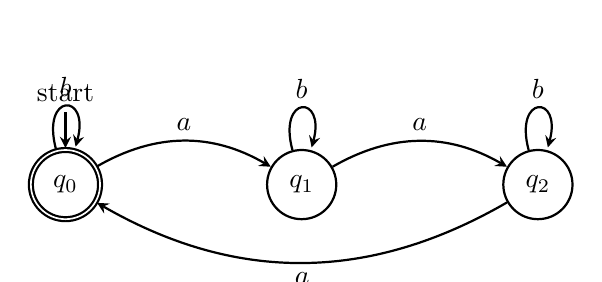
\begin{tikzpicture}[>=stealth, node distance=3cm, auto, thick]
    \node[state, initial above, accepting] (q0) {$q_0$};
    \node[state, right of=q0] (q1) {$q_1$};
    \node[state, right of=q1] (q2) {$q_2$};

    \draw[->] (q0) edge[loop above] node{$b$} (q0)
              (q0) edge[bend left] node{$a$} (q1)
    ;
    \draw[->] (q1) edge[loop above] node{$b$} (q1)
              (q1) edge[bend left] node{$a$} (q2)
    ;
    \draw[->] (q2) edge[loop above] node{$b$} (q2)
              (q2) edge[bend left] node{$a$} (q0)
    ;
\end{tikzpicture}
\end{center}

\textbf{转换函数表：}
\[
\begin{array}{c|cc}
\text{状态} & a & b \\
\hline
\to^* q_0 & q_1 & q_0 \\
q_1 & q_2 & q_1 \\
q_2 & q_0 & q_2
\end{array}
\]

验证：对于任意输入串，$q_0 \xrightarrow{*} q_i$当且仅当其中$a$的个数 $\equiv i \pmod 3$。仅当最终状态为$q_0$时接受。

\subsection{第2题（20分）：LL(1)分析}

文法G1：
\begin{align*}
S &\to A B a \\
A &\to A b \mid \varepsilon \\
B &\to d B \mid c
\end{align*}

\subsubsection*{2.1 句子 $bddca$ 的分析树（2分）}

推导过程：$S \Rightarrow ABa \Rightarrow Ab\;B\;a \Rightarrow b\;B\;a \Rightarrow b\;dB\;a \Rightarrow b\;d\;dB\;a \Rightarrow b\;d\;d\;c\;a$

\begin{center}
\begin{forest}
for tree={l sep=0.8cm, s sep=0.5cm}
[S
  [A
    [A [$\varepsilon$]]
    [$b$]
  ]
  [B
    [$d$]
    [B
      [$d$]
      [B [$c$]]
    ]
  ]
  [$a$]
]
\end{forest}
\end{center}

\subsubsection*{2.2 改写为G2（2分）}

G1中$A \to Ab$存在\textbf{直接左递归}，不适合自顶向下分析。

\textbf{消除左递归：} $A \to Ab \mid \varepsilon$ 等价于 $A \to bA \mid \varepsilon$（这两者都产生语言$\{b^n \mid n \ge 0\}$）。

\textbf{等价文法G2：}
\[
\boxed{
\begin{aligned}
(1)\; S &\to A B a \\
(2)\; A &\to b A \\
(3)\; A &\to \varepsilon \\
(4)\; B &\to d B \\
(5)\; B &\to c
\end{aligned}}
\]

\subsubsection*{2.3 FIRST与FOLLOW集（4分）}

\textbf{FIRST集：}
\begin{align*}
\text{FIRST}(A) &= \{b, \varepsilon\} \quad (\text{由}A \to bA\text{得}b\text{，由}A\to\varepsilon\text{得}\varepsilon) \\
\text{FIRST}(B) &= \{d, c\} \quad (\text{由}B\to dB\text{和}B\to c) \\
\text{FIRST}(S) &= (\text{FIRST}(A) \setminus \{\varepsilon\}) \cup \text{FIRST}(B) \\
                &= \{b\} \cup \{d, c\} = \{b, d, c\}
\end{align*}

\textbf{FOLLOW集：}（设$\$$为结束符）
\begin{align*}
\text{FOLLOW}(S) &= \{\$\} \\
\text{FOLLOW}(A) &= \text{FIRST}(Ba) \setminus \{\varepsilon\} = \{d, c\} \\
\text{FOLLOW}(B) &= \{a\}
\end{align*}
其中$\text{FOLLOW}(A)=\{d,c\}$是因为在$S \to ABa$中$A$后跟$B$，而$B$不能推导出$\varepsilon$（$B \to dB \mid c$均推导出至少一个终结符），故$\text{FIRST}(Ba)=\text{FIRST}(B)=\{d,c\}$。$\text{FOLLOW}(B)=\{a\}$是因为在$S \to ABa$中$B$后跟$a$。$\square$

\begin{center}
\begin{tabular}{c|c|c}
非终结符 & FIRST & FOLLOW \\
\hline
$S$ & $\{b, d, c\}$ & $\{\$\}$ \\
$A$ & $\{b, \varepsilon\}$ & $\{d, c\}$ \\
$B$ & $\{d, c\}$ & $\{a\}$ \\
\end{tabular}
\end{center}

\subsubsection*{2.4 LL(1)分析表（6分）}

对于每个产生式：
\begin{itemize}
    \item 对于 $A \to \alpha$，将产生式填入表中$[A, a]$位置，$\forall a \in \text{FIRST}(\alpha)$
    \item 若 $\varepsilon \in \text{FIRST}(\alpha)$，则$\forall b \in \text{FOLLOW}(A)$，在$[A, b]$处填入
\end{itemize}

\textbf{LL(1)分析表：}

\[
\begin{array}{c|ccccc}
     & a & b & c & d & \$ \\
\hline
S &   & S \to ABa & S \to ABa & S \to ABa &   \\
A &   & A \to bA  & A \to \varepsilon & A \to \varepsilon &   \\
B &   &     & B \to c   & B \to dB  &   \\
\end{array}
\]

\textbf{判断：G2是LL(1)文法。}

原因：分析表中每个格子至多只有一个产生式，无冲突：
\begin{itemize}
    \item $S$：$b, c, d$列各有唯一产生式，无冲突
    \item $A$：$b$列为$A \to bA$，$c, d$列为$A \to \varepsilon$，$\text{FIRST}(bA) \cap \text{FOLLOW}(A) = \{b\} \cap \{d,c\} = \varnothing$，无冲突
    \item $B$：$c$列为$B \to c$，$d$列为$B \to dB$，$\text{FIRST}(c) \cap \text{FIRST}(dB) = \{c\} \cap \{d\} = \varnothing$，无冲突
\end{itemize}

\subsubsection*{2.5 输入串 $bddca$ 的LL(1)分析过程（6分）}

约定：栈顶在左侧，推导时弹出栈顶非终结符，将产生式右部\textbf{逆序}压入（最左符号在栈顶）。

\begin{center}
\begin{tabular}{c|c|c|c}
\textbf{Step \#} & \textbf{Stack (top left)} & \textbf{Input} & \textbf{Action} \\
\hline
0 & $S\$$ & $bddca\$$ & --- \\
1 & $A B a\$$ & $bddca\$$ & $S \to ABa$ \\
2 & $b A B a\$$ & $bddca\$$ & $A \to bA$ \\
3 & $A B a\$$ & $ddca\$$ & match $b$ \\
4 & $B a\$$ & $ddca\$$ & $A \to \varepsilon$ \\
5 & $d B a\$$ & $ddca\$$ & $B \to dB$ \\
6 & $B a\$$ & $dca\$$ & match $d$ \\
7 & $d B a\$$ & $dca\$$ & $B \to dB$ \\
8 & $B a\$$ & $ca\$$ & match $d$ \\
9 & $c a\$$ & $ca\$$ & $B \to c$ \\
10 & $a\$$ & $a\$$ & match $c$ \\
11 & $\$$ & $\$$ & match $a$ / \textbf{ACCEPT} \\
\end{tabular}
\end{center}

分析成功，句子 $bddca$ 被接受。$\square$


\subsection{第3题（25分）：LR分析}

\textbf{已知文法：}
\begin{align*}
\text{G1:}\quad S &\to E + T &
E &\to (E) \mid a &
T &\to b \\
\text{G2:}\quad S &\to E + T &
E &\to (E) \mid a &
T &\to b \mid bE
\end{align*}

\subsubsection*{3.1 G1的拓广文法G3（1分）}

引入新的开始符号$S'$和产生式$S' \to S$：

\[
\boxed{
\begin{aligned}
(0)\; S' &\to S \\
(1)\; S  &\to E + T \\
(2)\; E  &\to (\,E\,) \\
(3)\; E  &\to a \\
(4)\; T  &\to b
\end{aligned}}
\]

\subsubsection*{3.2 LR(0)项目集规范族（活前缀DFA）（6分）}

\textbf{约定：}大写字母为非终结符，$\text{goto}(I_i, X) = I_j$表示从状态$I_i$经符号$X$到达状态$I_j$。

\begin{align*}
I_0 &= \text{closure}(\{[S' \to \bullet S]\}) \\
    &= \{ S' \to \bullet S,\; S \to \bullet E + T,\; E \to \bullet (E),\; E \to \bullet a \} \\[4pt]
I_1 &= \text{goto}(I_0, S) = \{ S' \to S\bullet \} \quad (\text{接受状态}) \\[4pt]
I_2 &= \text{goto}(I_0, E) = \{ S \to E\bullet + T \} \\[4pt]
I_3 &= \text{goto}(I_0, (\;) = \{ E \to (\bullet E),\; E \to \bullet (E),\; E \to \bullet a \} \\[4pt]
I_4 &= \text{goto}(I_0, a) = \{ E \to a\bullet \} \quad (\text{归约状态，用产生式(3)}) \\[4pt]
I_5 &= \text{goto}(I_2, +) = \{ S \to E + \bullet T,\; T \to \bullet b \} \\[4pt]
I_6 &= \text{goto}(I_5, T) = \{ S \to E + T\bullet \} \quad (\text{归约状态，用产生式(1)}) \\[4pt]
I_7 &= \text{goto}(I_5, b) = \{ T \to b\bullet \} \quad (\text{归约状态，用产生式(4)}) \\[4pt]
I_8 &= \text{goto}(I_3, E) = \{ E \to (E\bullet) \} \\[4pt]
I_9 &= \text{goto}(I_8, )\;) = \{ E \to (E)\bullet \} \quad (\text{归约状态，用产生式(2)})
\end{align*}

\textbf{状态转移关系：}
\[
\begin{aligned}
I_0 &\xrightarrow{S} I_1,\; I_0 \xrightarrow{E} I_2,\; I_0 \xrightarrow{(} I_3,\; I_0 \xrightarrow{a} I_4 \\
I_2 &\xrightarrow{+} I_5 \\
I_3 &\xrightarrow{E} I_8,\; I_3 \xrightarrow{(} I_3,\; I_3 \xrightarrow{a} I_4 \\
I_5 &\xrightarrow{T} I_6,\; I_5 \xrightarrow{b} I_7 \\
I_8 &\xrightarrow{)} I_9
\end{aligned}
\]

\textbf{活前缀DFA图示：}
\begin{center}
\begin{tikzpicture}[>=stealth, node distance=2cm and 2.2cm, on grid, auto, scale=0.88,
    every state/.style={minimum size=8.5mm}]
\node[state] (I0) {$I_0$};
\node[state, above right=0.8cm and 2cm of I0] (I1) {$I_1$};
\node[state, right=of I0] (I2) {$I_2$};
\node[state, below=of I0] (I3) {$I_3$};
\node[state, left=of I3] (I4) {$I_4$};
\node[state, right=of I2] (I5) {$I_5$};
\node[state, right=of I5] (I6) {$I_6$};
\node[state, below=of I5] (I7) {$I_7$};
\node[state, below=of I3] (I8) {$I_8$};
\node[state, below=of I8] (I9) {$I_9$};

\draw[->] (I0) -- node[above left]{$S$} (I1);
\draw[->] (I0) -- node[above]{$E$} (I2);
\draw[->] (I0) -- node[left]{$($} (I3);
\draw[->] (I0) -- node[above]{$a$} (I4);
\draw[->] (I2) -- node[above]{$+$} (I5);
\draw[->] (I5) -- node[above]{$T$} (I6);
\draw[->] (I5) -- node[left]{$b$} (I7);
\draw[->] (I3) -- node[left]{$E$} (I8);
\draw[->] (I3) edge[loop left] node{$($} (I3);
\draw[->] (I3) -- node[above]{$a$} (I4);
\draw[->] (I8) -- node[left]{$)$} (I9);
\end{tikzpicture}
\end{center}

\subsubsection*{3.3 LR(0)分析表（5分）}

\[
\begin{array}{c|cccccc|ccc}
\multirow{2}{*}{\textbf{State}} & \multicolumn{6}{c|}{\textbf{ACTION}} & \multicolumn{3}{c}{\textbf{GOTO}} \\
     & a   & b   & (   & )   & +   & \$   & S & E & T \\
\hline
0    & s4  &     & s3  &     &     &      & 1 & 2 &   \\
1    &     &     &     &     &     & acc  &   &   &   \\
2    &     &     &     &     & s5  &      &   &   &   \\
3    & s4  &     & s3  &     &     &      &   & 8 &   \\
4    & r3  & r3  & r3  & r3  & r3  & r3   &   &   &   \\
5    &     & s7  &     &     &     &      &   &   & 6 \\
6    & r1  & r1  & r1  & r1  & r1  & r1   &   &   &   \\
7    & r4  & r4  & r4  & r4  & r4  & r4   &   &   &   \\
8    &     &     &     & s9  &     &      &   &   &   \\
9    & r2  & r2  & r2  & r2  & r2  & r2   &   &   &   \\
\end{array}
\]

说明：$sX$表示移进到状态$X$，$rX$表示按产生式$X$归约，$gX$表示GOTO状态$X$。

\subsubsection*{3.4 输入串 $(a)+b$ 的LR分析过程（5分）}

约定：符号栈和状态栈各自维护，GOTO只在归约后使用。

\begin{center}
\footnotesize
\begin{tabular}{c|c|c|c}
\textbf{Step} & \textbf{Stack (Symbols / States)} & \textbf{Input} & \textbf{Action} \\
\hline
0  & \$ $\mid$ 0                   & $(a)+b\,\$ $ & shift $($, goto 3 \\
1  & \$ ( $\mid$ 0 3                & $a)+b\,\$ $  & shift $a$, goto 4 \\
2  & \$ ( a $\mid$ 0 3 4            & $)+b\,\$ $   & reduce by (3) $E \to a$ \\
3  & \$ ( E $\mid$ 0 3 8            & $)+b\,\$ $   & shift $)$, goto 9 \\
4  & \$ ( E ) $\mid$ 0 3 8 9        & $+b\,\$ $    & reduce by (2) $E \to (E)$ \\
5  & \$ E $\mid$ 0 2                & $+b\,\$ $    & shift $+$, goto 5 \\
6  & \$ E + $\mid$ 0 2 5            & $b\,\$ $     & shift $b$, goto 7 \\
7  & \$ E + b $\mid$ 0 2 5 7        & $\,\$ $      & reduce by (4) $T \to b$ \\
8  & \$ E + T $\mid$ 0 2 5 6        & $\,\$ $      & reduce by (1) $S \to E + T$ \\
9  & \$ S $\mid$ 0 1                & $\,\$ $      & \textbf{ACCEPT} \\
\end{tabular}
\end{center}

分析成功，输入串 $(a)+b$ 被接受。$\square$

\textbf{Step 3 详解（归约 $E \to a$）：}
状态4为$\{E \to a\bullet\}$，执行归约：弹出1个符号（$a$）和1个状态（4），栈顶变为状态3。$\text{goto}(I_3, E) = I_8$，压入$E$和状态8。

\textbf{Step 4 详解（归约 $E \to (E)$）：}
状态9为$\{E \to (E)\bullet\}$，执行归约：弹出3个符号$), E, ($和3个状态9, 8, 3。栈顶变为状态0。$\text{goto}(I_0, E) = I_2$，压入$E$和状态2。

\subsubsection*{3.5 G2的状态$I_8$冲突分析（4分）}

\textbf{G2的LR(0)项目集状态$I_8$：}
\[
\begin{aligned}
T &\to b\bullet \quad \text{（归约项目：按}T \to b\text{归约）} \\
T &\to b\bullet E \quad \text{（移进项目：期望移进}E\text{的FIRST集符号）} \\
E &\to \bullet (E) \\
E &\to \bullet a
\end{aligned}
\]

\textbf{LR(0)中是否存在冲突？}

\textbf{是的，存在移进--归约冲突。} $T \to b\bullet$要求归约，而$T \to b\bullet E$（以及$E$的闭包）要求移进$($或$a$。LR(0)不考虑前瞻符，无法区分应该归约还是移进。

\textbf{SLR(1)能否解决？}

\textbf{可以解决。} SLR(1)在决定是否归约$T \to b$时，只在输入符号属于$\text{FOLLOW}(T)$时才归约。

计算$\text{FOLLOW}(T)$（G2中）：
\begin{itemize}
    \item 从$S \to E + T$：$T$后面是\$（或$\text{FOLLOW}(S)$），故$\$ \in \text{FOLLOW}(T)$
    \item 从$T \to bE$：$T$是左部，不贡献FOLLOW
    \item $T$不出现在其他产生式的右部
\end{itemize}
故 $\text{FOLLOW}(T) = \{\$\}$。

在SLR(1)中，状态$I_8$的归约动作$T \to b$仅在输入为$\$ $时才执行。而移进动作仅在输入为$($或$a$（$\in \text{FIRST}(E)$）时才执行。由于$\{\$\} \cap \{(, a\} = \varnothing$，没有交集，冲突被消除。

\textbf{结论：SLR(1)可以解决该冲突。}

\subsubsection*{3.6 LR(1)的改进原理与闭包计算方法（4分）}

\textbf{一、LR(1)项目是什么？}

LR(1)项目形如 $[A \to \alpha \bullet \beta,\; a]$，包含两部分：
\begin{itemize}
    \item \textbf{核心部分} $A \to \alpha \bullet \beta$：与 LR(0) 项目相同，表示已看到 $\alpha$、期望看到 $\beta$
    \item \textbf{前瞻符（lookahead）} $a$：一个终结符，表示\textbf{只有当}当前输入符号是 $a$ 时，才允许按此项目归约（当 $\beta = \varepsilon$ 时）
\end{itemize}

举例：$[E \to \bullet (E),\; +]$ 的含义是"我们在期望规约一个 $E$，而且这个 $E$ 的右侧必须紧跟着一个 $+$"。

\textbf{二、LR(1) 为什么比 SLR(1) 更精确？}

SLR(1) 对产生式 $A \to \gamma$ 的\textbf{所有出现}统一使用 $\text{FOLLOW}(A)$ 来决定何时归约。但 $A$ 可能在文法的不同上下文中出现，不同上下文中 $A$ 后面能跟的符号是不同的。SLR(1) 把所有这些可能混在一起，导致不精确。

LR(1) 给\textbf{每个项目单独}附加一个精确的前瞻符。同一个产生式 $A \to \gamma$ 在不同上下文中可能带不同的前瞻符，从而只在正确的上下文中归约。

\textbf{三、闭包计算的通用方法}

LR(1) 闭包的计算是 LR(1) 最核心的算法。从初始项目集出发，反复应用以下规则直到不再产生新项目：

\begin{center}
\fbox{
\begin{minipage}{0.88\textwidth}
\textbf{闭包扩展规则：}

若状态中存在项目 $[A \to \alpha \bullet B \beta,\; a]$（即 $\bullet$ 后面是一个非终结符 $B$），
则对 $B$ 的每个产生式 $B \to \gamma$，向该状态添加项目：
\[
[B \to \bullet \gamma,\; b], \quad \text{其中 } b \in \text{FIRST}(\beta a)
\]
\end{minipage}
}
\end{center}

\textbf{关键问题：为什么前瞻符是 $\text{FIRST}(\beta a)$？}

在项目 $[A \to \alpha \bullet B \beta,\; a]$ 中：
\begin{itemize}
    \item 我们期望接下来看到 $B$（由产生式 $B \to \gamma$ 推导）
    \item $B$ 推导完毕后，后面紧跟着的是 $\beta$（如果 $\beta \neq \varepsilon$）或 $a$（如果 $\beta$ 能推导出 $\varepsilon$）
    \item 因此，当我们最终归约 $B \to \gamma$ 时，当前输入符号必须是 $\text{FIRST}(\beta a)$ 中的某个符号
    \item 这个符号就被设置为新项目 $[B \to \bullet \gamma,\; b]$ 的前瞻符
\end{itemize}

\textbf{四、以 G2 为例，逐步推导初始状态 $I_0$}

G2 拓广后：
\[
\begin{aligned}
(0)\; S' &\to S \\
(1)\; S  &\to E + T \\
(2)\; E  &\to (E) \\
(3)\; E  &\to a \\
(4)\; T  &\to b \\
(5)\; T  &\to bE
\end{aligned}
\]

\textbf{第1步：放入种子项目。}
LR(1) DFA 的初始状态始终从 $[S' \to \bullet S,\; \$]$ 开始，表示"期望看到 $S$，然后文件结束"。
\[
I_0 = \{\; [S' \to \bullet S,\; \$] \;\}
\]

\textbf{第2步：闭包扩展（第1轮）。}
检查 $[S' \to \bullet S,\; \$]$：$\bullet$ 后面是 $S$（非终结符），触发扩展。

对 $S$ 的产生式 $S \to E + T$，计算前瞻符：
\begin{itemize}
    \item 在 $S' \to \bullet S$ 中，$B = S$，$\beta = \varepsilon$（$S$ 后面什么都没有），$a = \$$
    \item 所以前瞻符 $b \in \text{FIRST}(\varepsilon \cdot \$) = \text{FIRST}(\$) = \{\$\}$
\end{itemize}
添加：$[S \to \bullet E + T,\; \$]$

现在 $I_0 = \{\; [S' \to \bullet S,\; \$],\; [S \to \bullet E + T,\; \$] \;\}$

\textbf{第3步：闭包扩展（第2轮）。}
检查新项目 $[S \to \bullet E + T,\; \$]$：$\bullet$ 后面是 $E$（非终结符），触发扩展。

对 $E$ 的产生式 $E \to (E)$ 和 $E \to a$，计算前瞻符：
\begin{itemize}
    \item 在 $S \to \bullet E + T$ 中，$B = E$，$\beta = +T$，$a = \$$
    \item 前瞻符 $b \in \text{FIRST}(+T \cdot \$) = \text{FIRST}(+T) = \{+\}$
    \item 解释：归约出 $E$ 之后，后面应该跟着 $+T\$ $，所以紧跟着的第一个符号必须是 $+$
\end{itemize}
添加：$[E \to \bullet (E),\; +]$ 和 $[E \to \bullet a,\; +]$

\textbf{第4步：检查是否还有新项目需扩展。}
新添加的项目 $[E \to \bullet (E),\; +]$ 的 $\bullet$ 后面是 $($（终结符），不触发扩展。
$[E \to \bullet a,\; +]$ 的 $\bullet$ 后面是 $a$（终结符），也不触发扩展。

闭包计算结束。最终：
\[
\boxed{
I_0 = \left\{
\begin{aligned}
&[S' \to \bullet S,\; \$],\\
&[S  \to \bullet E + T,\; \$],\\
&[E  \to \bullet (E),\; +],\\
&[E  \to \bullet a,\; +]
\end{aligned}
\right\}
}
\]

\textbf{五、前瞻符的意义——一个具体对比}

假设后续分析中，从 $I_0$ 经移进和归约到达了含 $[E \to a\bullet,\; +]$ 的状态。此时：
\begin{itemize}
    \item \textbf{SLR(1) 的做法：} 查 $\text{FOLLOW}(E)$。在 G2 中，$E$ 出现在 $S \to E+T$（后跟 $+$）和 $E \to (E)$（后跟 $)$）中，故 $\text{FOLLOW}(E) = \{+, )\}$。SLR(1) 在输入为 $+$ \textbf{或} $)$ 时都按 $E \to a$ 归约。但如果输入是 $)$，归约 $E \to a$ 可能是错误的——因为我们当前所在的上下文可能不允许 $E$ 后面跟 $)$。
    \item \textbf{LR(1) 的做法：} 直接看前瞻符。这个项目的 lookahead 是 $+$，所以\textbf{只在}输入为 $+$ 时才归约。输入为 $)$ 时不会错误归约。
\end{itemize}

这就是 LR(1) 比 SLR(1) 强大的本质：每个项目带着自己精确的"触发条件"，而不是用一个笼统的 FOLLOW 集。

\textbf{六、通用闭包算法（伪代码）}

\begin{center}
\fbox{
\begin{minipage}{0.88\textwidth}
\textbf{function} closure($I$):\\
\quad \textbf{repeat}:\\
\qquad \textbf{for each} item $[A \to \alpha \bullet B \beta,\; a]$ in $I$:\\
\qquad \qquad \textbf{for each} production $B \to \gamma$:\\
\qquad \qquad \qquad \textbf{for each} terminal $b \in \text{FIRST}(\beta a)$:\\
\qquad \qquad \qquad \qquad add $[B \to \bullet \gamma,\; b]$ to $I$\\
\quad \textbf{until} $I$ no longer changes\\
\quad \textbf{return} $I$
\end{minipage}
}
\end{center}

其中 $\text{FIRST}(\beta a)$ 的计算规则与标准 FIRST 集计算一致：
\begin{itemize}
    \item 若 $\beta = \varepsilon$，则 $\text{FIRST}(\varepsilon a) = \{a\}$：前瞻符直接继承自外层项目的 $a$
    \item 若 $\beta$ 非空，则依次取 $\beta$ 中各符号的 FIRST 集，直到遇到不能推导 $\varepsilon$ 的符号；若 $\beta$ 整体可推导 $\varepsilon$，最后还要并上 $\{a\}$
\end{itemize}

\textbf{七、与 SLR(1) 的对比总结}

\begin{center}
\begin{tabular}{p{0.38\textwidth}|p{0.55\textwidth}}
\textbf{SLR(1)} & \textbf{LR(1)} \\
\hline
归约条件：输入 $\in \text{FOLLOW}(A)$，对所有 $A \to \gamma$ 的项目统一使用 & 归约条件：输入 $= a$，其中 $a$ 是\textbf{该项目}的前瞻符 \\
\hline
前瞻符来源：$\text{FOLLOW}(A)$ 从整个文法的产生式中统计 & 前瞻符来源：通过闭包运算从上下文逐步计算，精确到每个出现位置 \\
\hline
状态数与 LR(0) 相同 & 状态数更多（同一个 LR(0) 核心可能因前瞻符不同而分裂为多个 LR(1) 状态） \\
\hline
能力较弱，部分文法无法处理 & 能力最强，LR(1) 文法严格包含 SLR(1) 文法 \\
\end{tabular}
\end{center}


\vfill
\begin{center}
\rule{0.3\textwidth}{0.4pt} \\
\textit{--- 解答完毕 ---}
\end{center}

\end{document}
